\renewcommand\thesection{\arabic{section}}
\renewcommand\thesubsection{\thesection.\arabic{subsection}}

\begin{figure}[ht]
    \begin{subfigure}[b]{0.3\textwidth}
        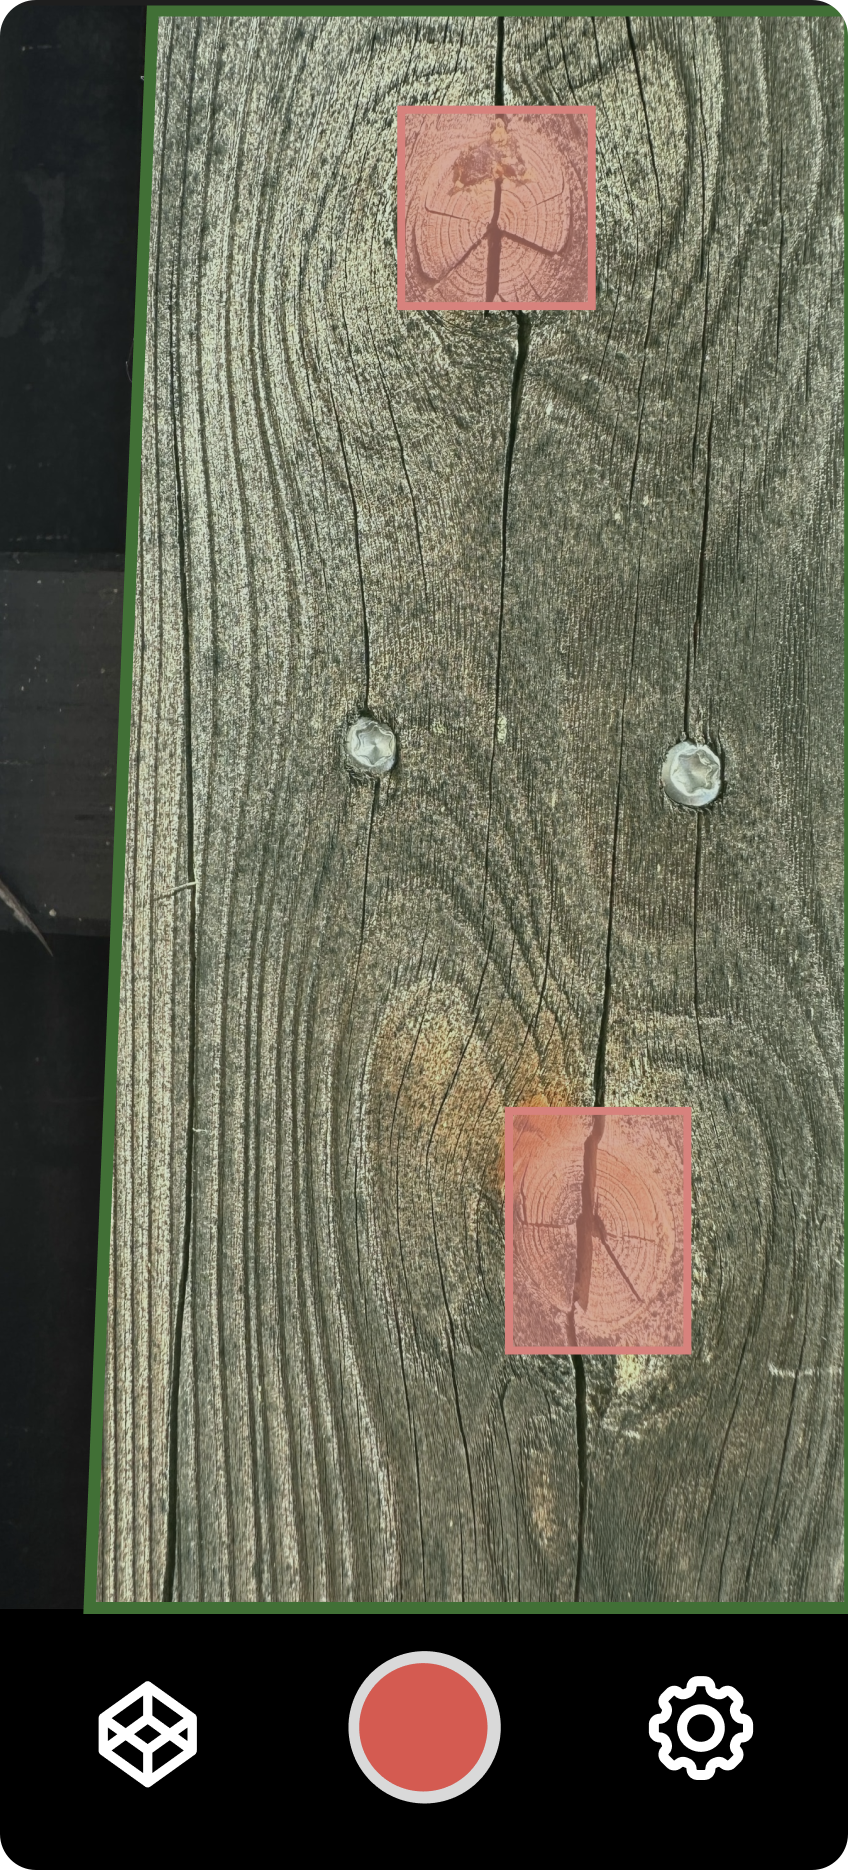
\includegraphics[width=0.7\textwidth]{Master Thesis/Images/Section_3/Mock/3-Mock3.png}
    \end{subfigure}
     \hfill
    \begin{subfigure}[b]{0.3\textwidth}
        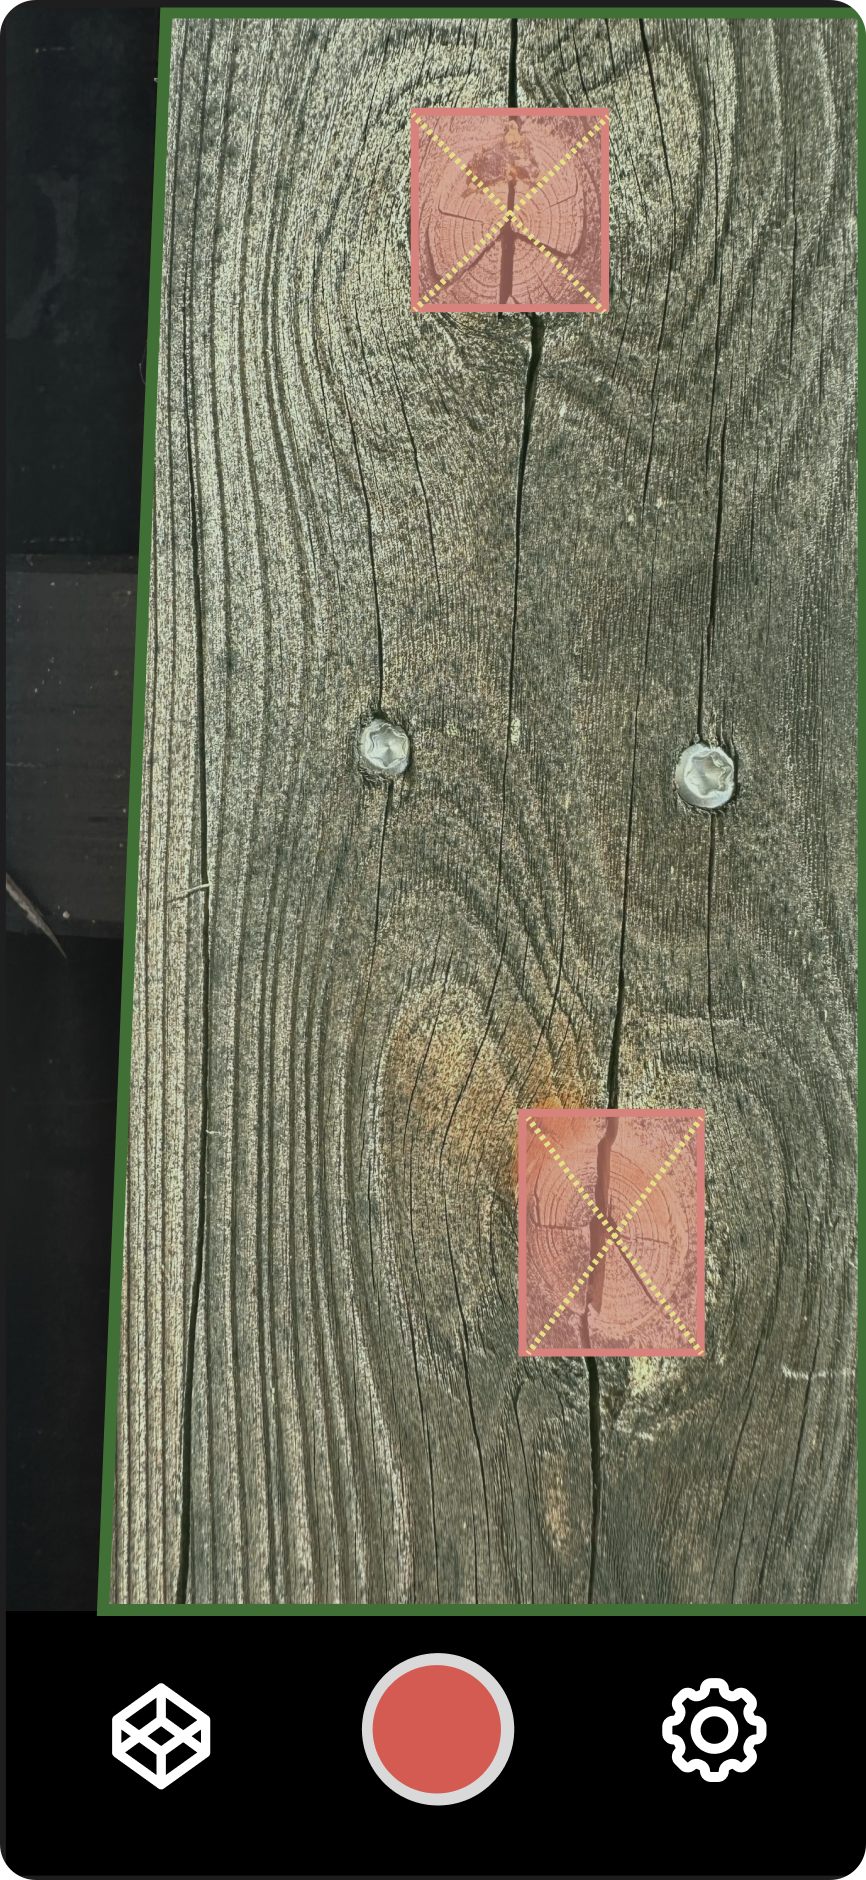
\includegraphics[width=0.7\textwidth]{Master Thesis/Images/Section_3/Mock/3-Mock4.png}
    \end{subfigure}
     \hfill
    \begin{subfigure}[b]{0.3\textwidth}
        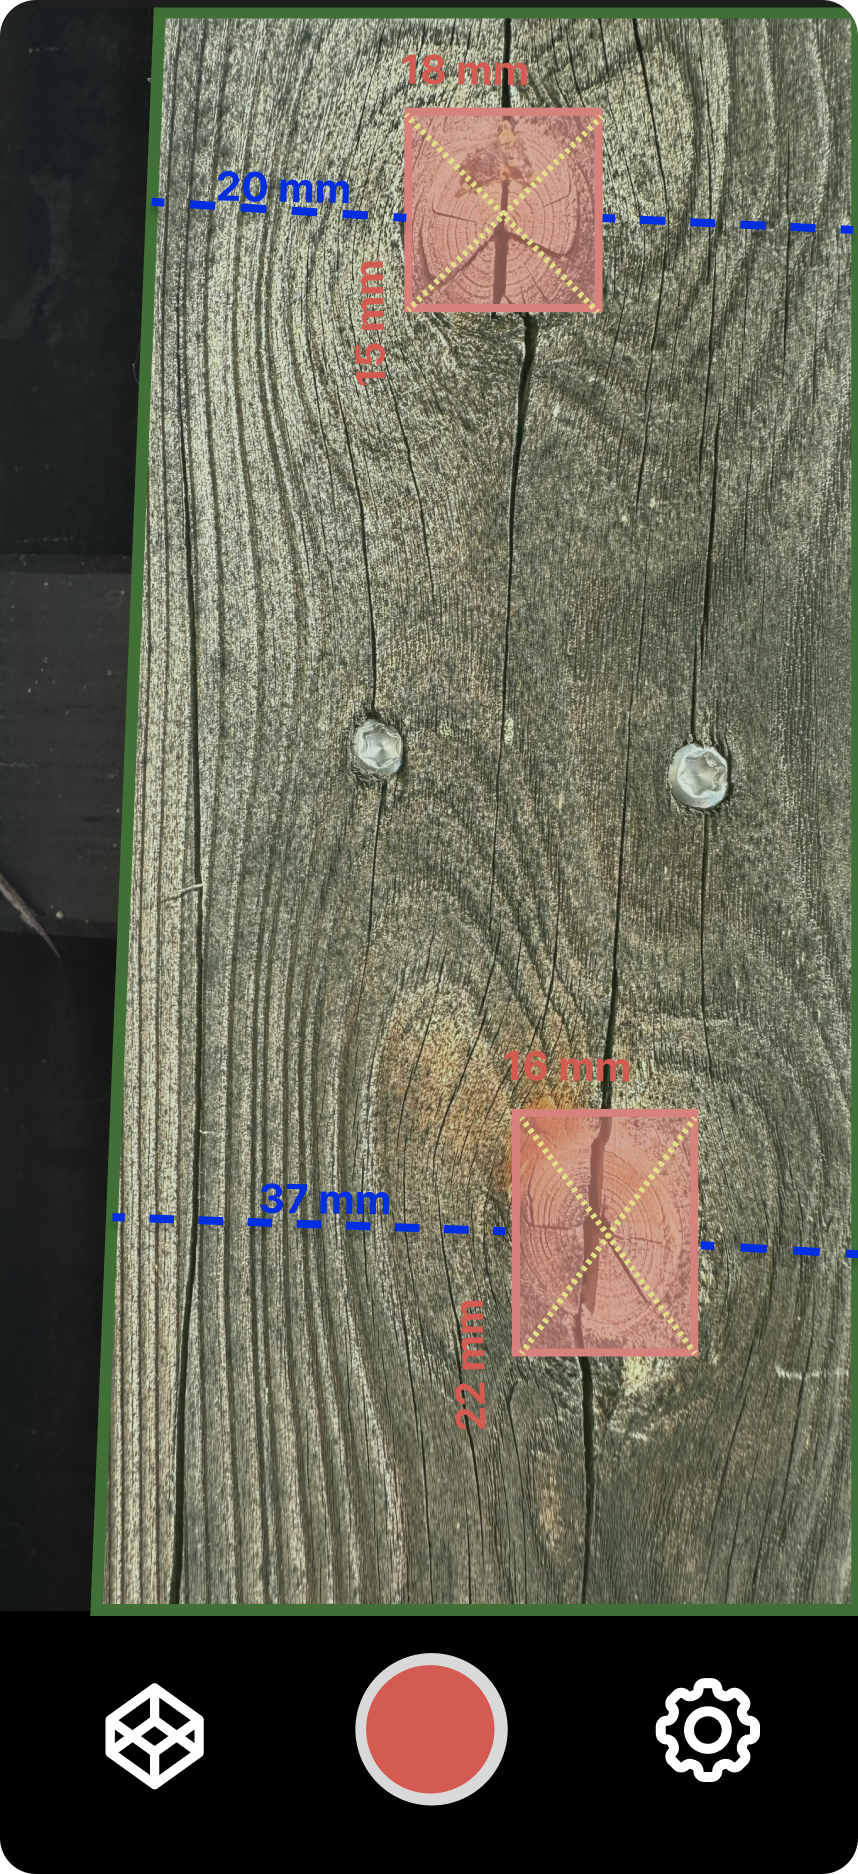
\includegraphics[width=0.7\textwidth]{Master Thesis/Images/Section_3/Mock/3-Mock5.png}
    \end{subfigure}
  \caption{Mocked-up output after dimension estimation of wood knots and distance to the boundary of wooden beams.}   
    \label{fig:mock3}
\end{figure}  


\textbf{Goal}:\\

In ideal situation, this step focus on the estimation of the dimension of wood knots assisted with the in-built iPhone Measure API and/or machine learning model to correctly calculate the exact size of the bounding box of detected wood knots in reality. Apple offers various API to access the data through sensors like lidar or Gyroscope. It is also possible to access the measurement API in iPhone supported by ARKit from Apple. (Figure~\ref{fig:iphone_mea}) Otherwise

\begin{figure}[ht]
  \centering
   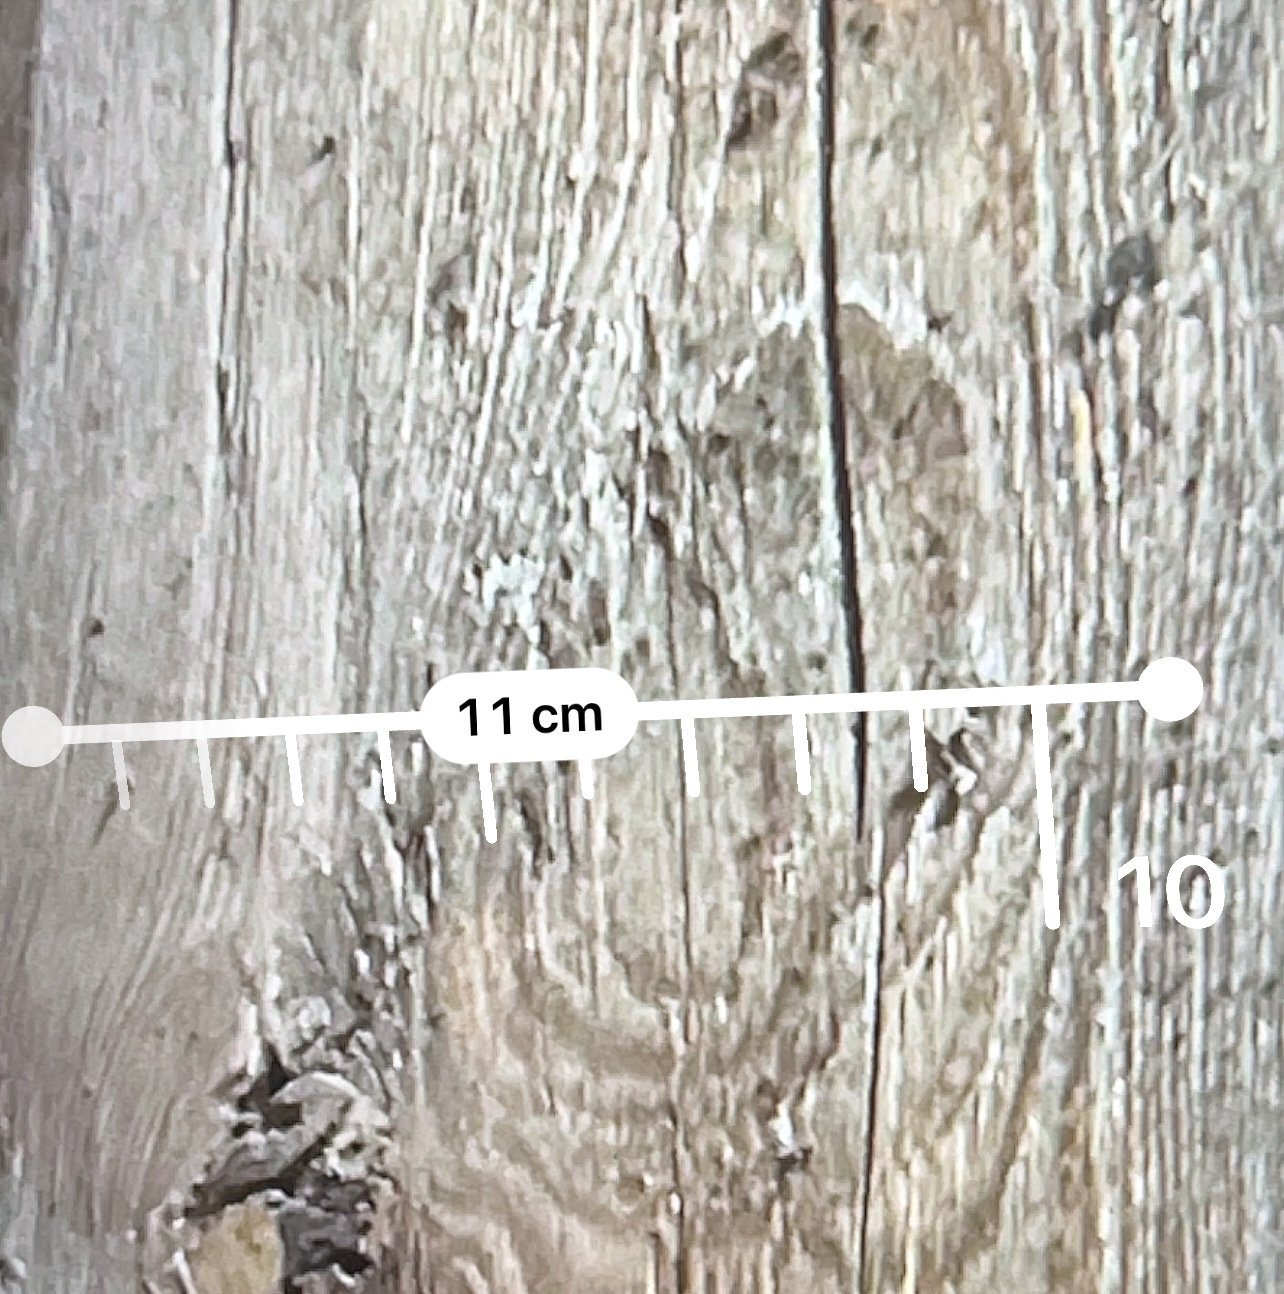
\includegraphics[width=.5\textwidth]{Master Thesis/Images/Section_3/3_iphone_measure.jpg}
  \caption{Mesurement using Measure App in iPhone}   
  \label{fig:iphone_mea}
\end{figure}  


\hspace*{\fill}

\textbf{Data set}:\\



\hspace*{\fill}

\textbf{Potential methods}:\\

aasdasdasd


\hspace*{\fill}

\textbf{Output}:\\

aasdasdasd

